% !TEX Root = ../defense.tex

\section[PhD Research]{PhD George Washington University}

\subsection[Asteroid Missions]{Asteroid Missions}

\begin{frame}{Asteroid Missions}
\begin{itemize}
    \item Science - insight into the early formation of the solar system
    \item Mining - vast quantities of useful materials
    \item Impact - high risk from hazardous near-Earth asteroids
\end{itemize}    

\begin{center}
    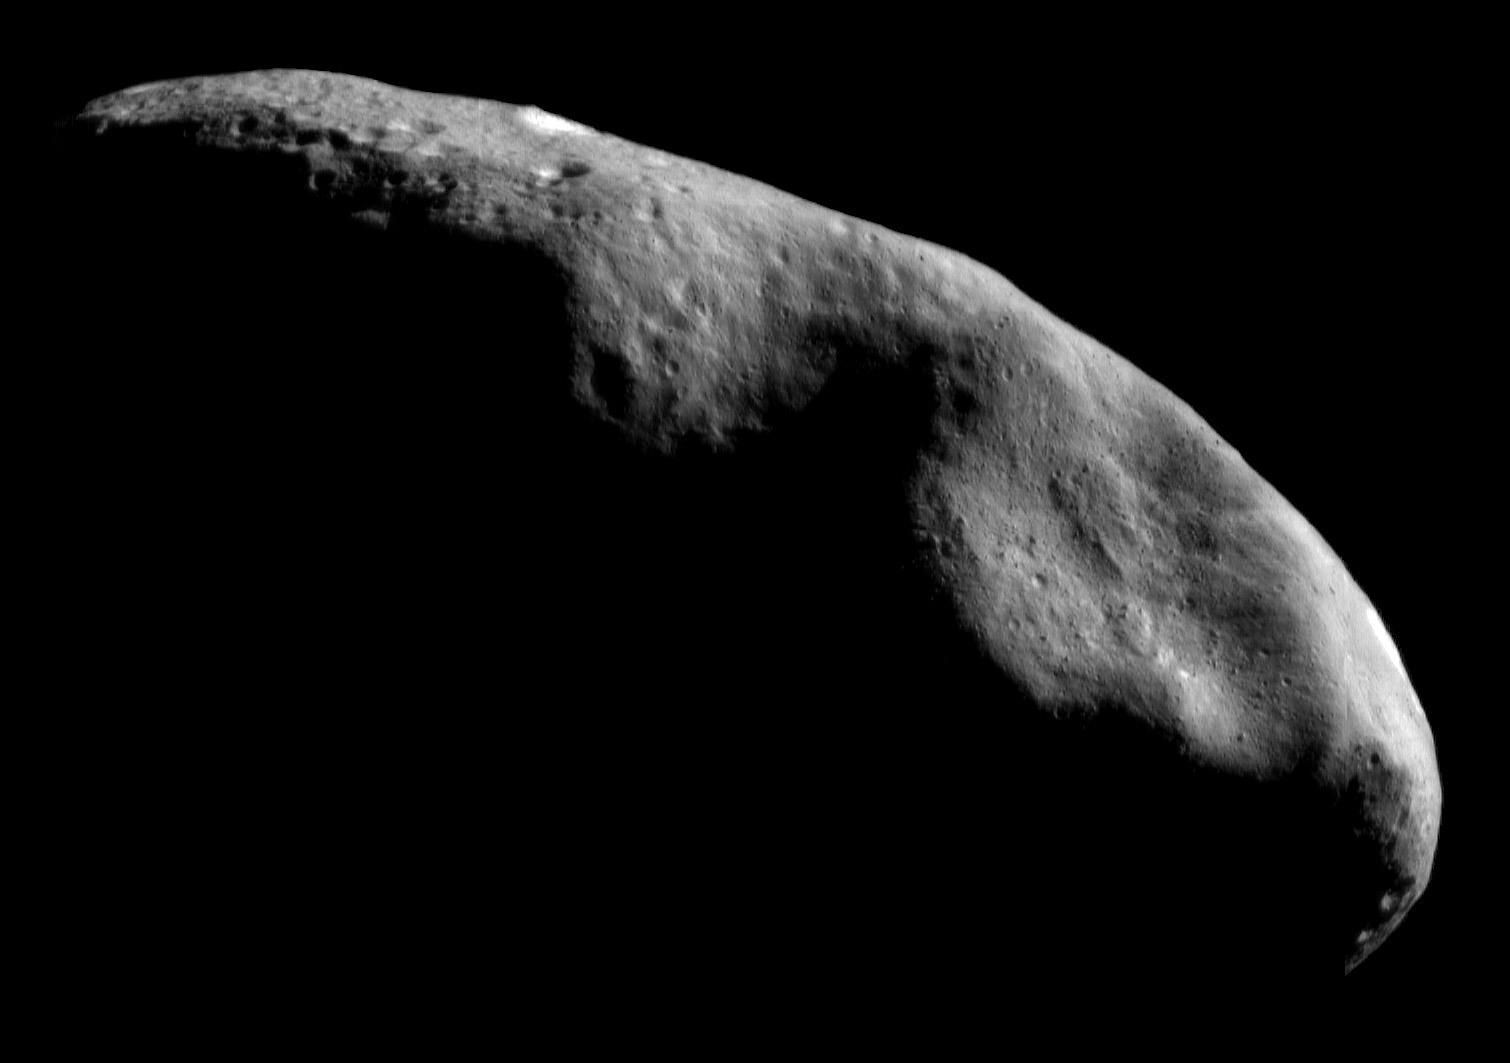
\includegraphics[height=0.5\textheight,width=0.5\textwidth,keepaspectratio]{figures/defense/near_mos_20001203_full.jpg}
    ~
    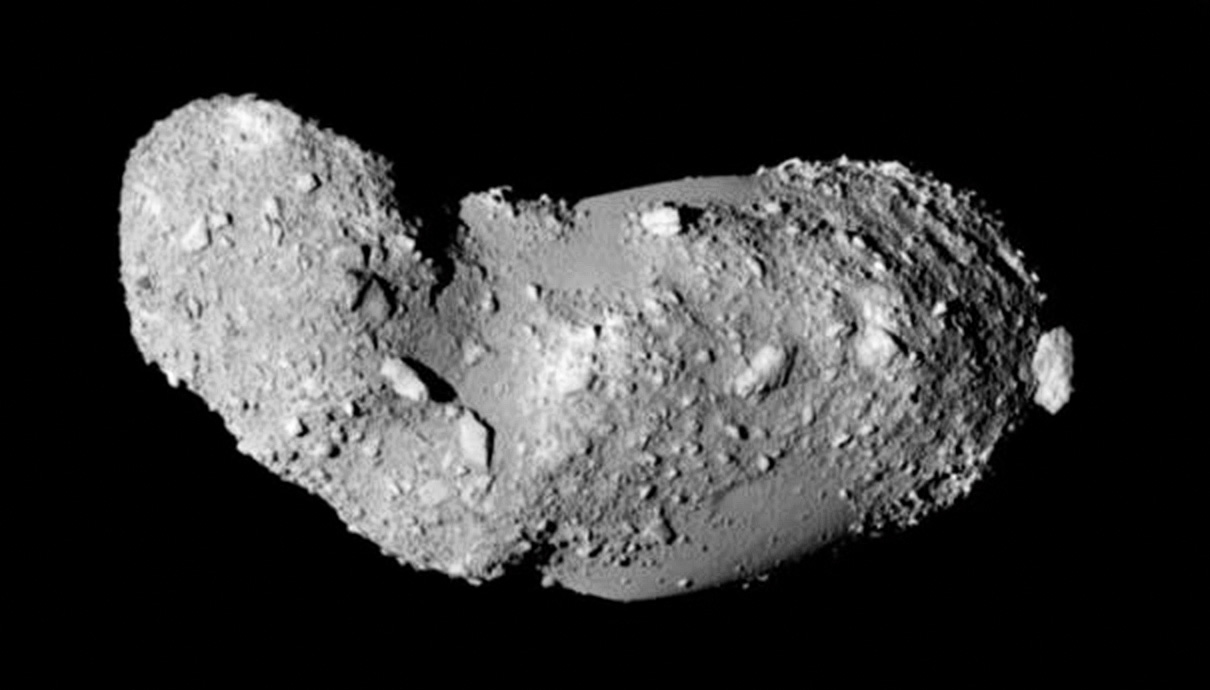
\includegraphics[height=0.5\textheight,width=0.5\textwidth,keepaspectratio]{figures/defense/Itokawa8_hayabusa_1210.jpg}
\end{center}
\end{frame}

\begin{frame}{Asteroid Mining}
    \begin{itemize}
      \item Useful materials can be extracted from asteroids to support:
      \begin{itemize}
          \item Propulsion, construction, life support, agriculture, and precious/strategic metals
      \end{itemize}
      \item Commercialization of near-Earth asteroids is feasible
    \end{itemize}

\pause

\begin{center}
\small
    \begin{tabular}{|l|r|r|}
        \hline 
        Element & Price (\SI{}{\$\per\kilo\gram}) & Sales (\SI{}{\$M\per yr}) \\
        \hline \hline 
        Phosphorous (P) & \num{0.08}  & \num{2167} \\
        Gallium (Ga) & \num{300.00}  & \num{1544} \\
        Germanium (Ge) & \num{745.00} & \num{6145} \\
        \hline \hline 
        Platinum (Pt) & \num{12394.00} & \num{1705} \\
        Gold (Au) & \num{12346.00} & \num{49} \\
        Osmium (Os) & \num{12860.00} & \num{307} \\
        \hline
    \end{tabular}
\end{center}

\end{frame}

\begin{frame}[t]{Problem statement}
    \begin{itemize}
        \item Ground based systems only provide a coarse shape estimate
        \item Spacecraft operations, e.g.\ landing, requires an accurate gravity model
        \item The gravity model accuracy is based on the accuracy of the shape
    \end{itemize}

    \begin{block}{}
        \begin{center}
            \begin{enumerate}
                \item Need an accurate shape before arrival
                \item Only in-situ measurements can provide the required detail
            \end{enumerate}
        \end{center}
    \end{block}
    
    This dissertation develops:
    \begin{enumerate}
        \item Correct dynamic model to predict motion of spacecraft,
        \item Control system to transfer around the small body,
        \item An efficient method to estimate and update the shape of the small body.
    \end{enumerate}
\end{frame}

\subsection[Electric Propulsion]{Electric Propulsion}  

\begin{frame} \label{slide:lowthrust_vehicles}%-----------------------------%
\frametitle{Low-thrust vehicles} % electric propulsion
\begin{itemize}
    \item Low-thrust orbital transfers offer increased mission oportunities
    \begin{itemize}
        \item Electric propulsion is increasing in capability
        \item Offers much higher specific impulse than chemical engines 
        \item Requires much longer operating periods for maneuvers 
        \item Enables long duration missions with frequent thrusting
    \end{itemize}
\end{itemize}

\begin{center}
    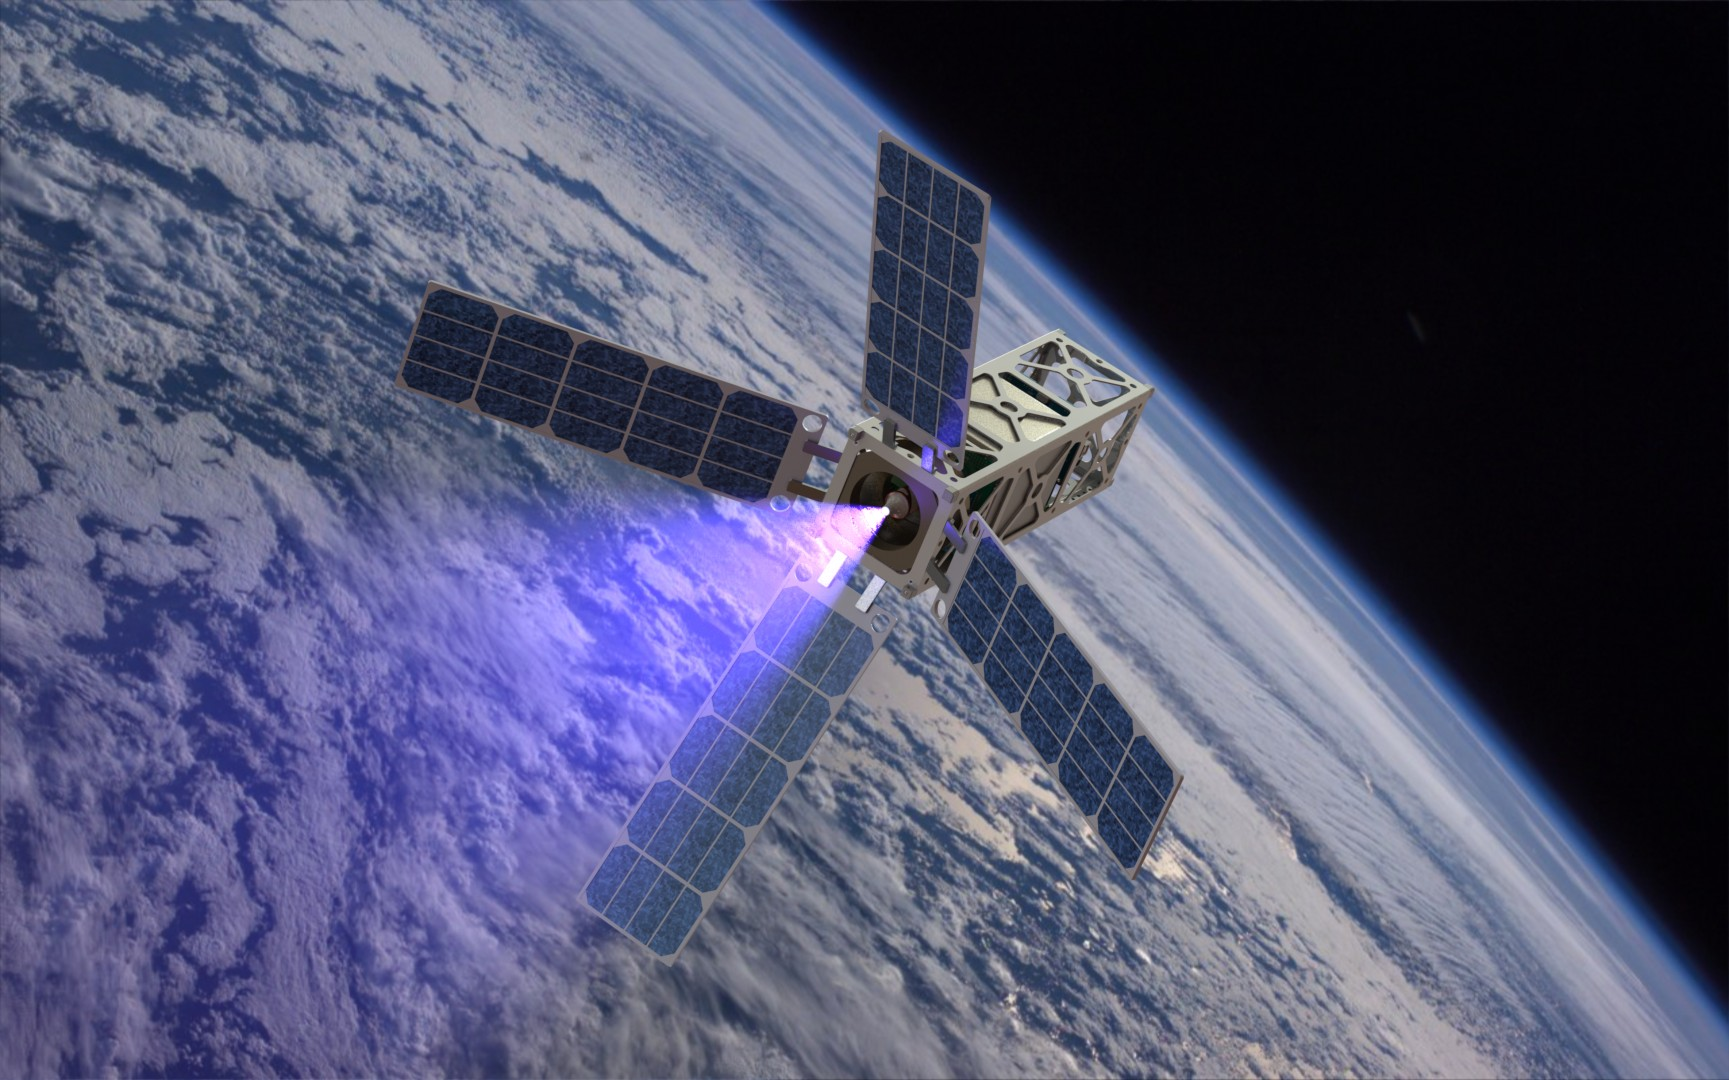
\includegraphics[height=0.4\textheight,width=0.5\textwidth,keepaspectratio]{figures/defense/patriot_plume.jpg}
    ~
    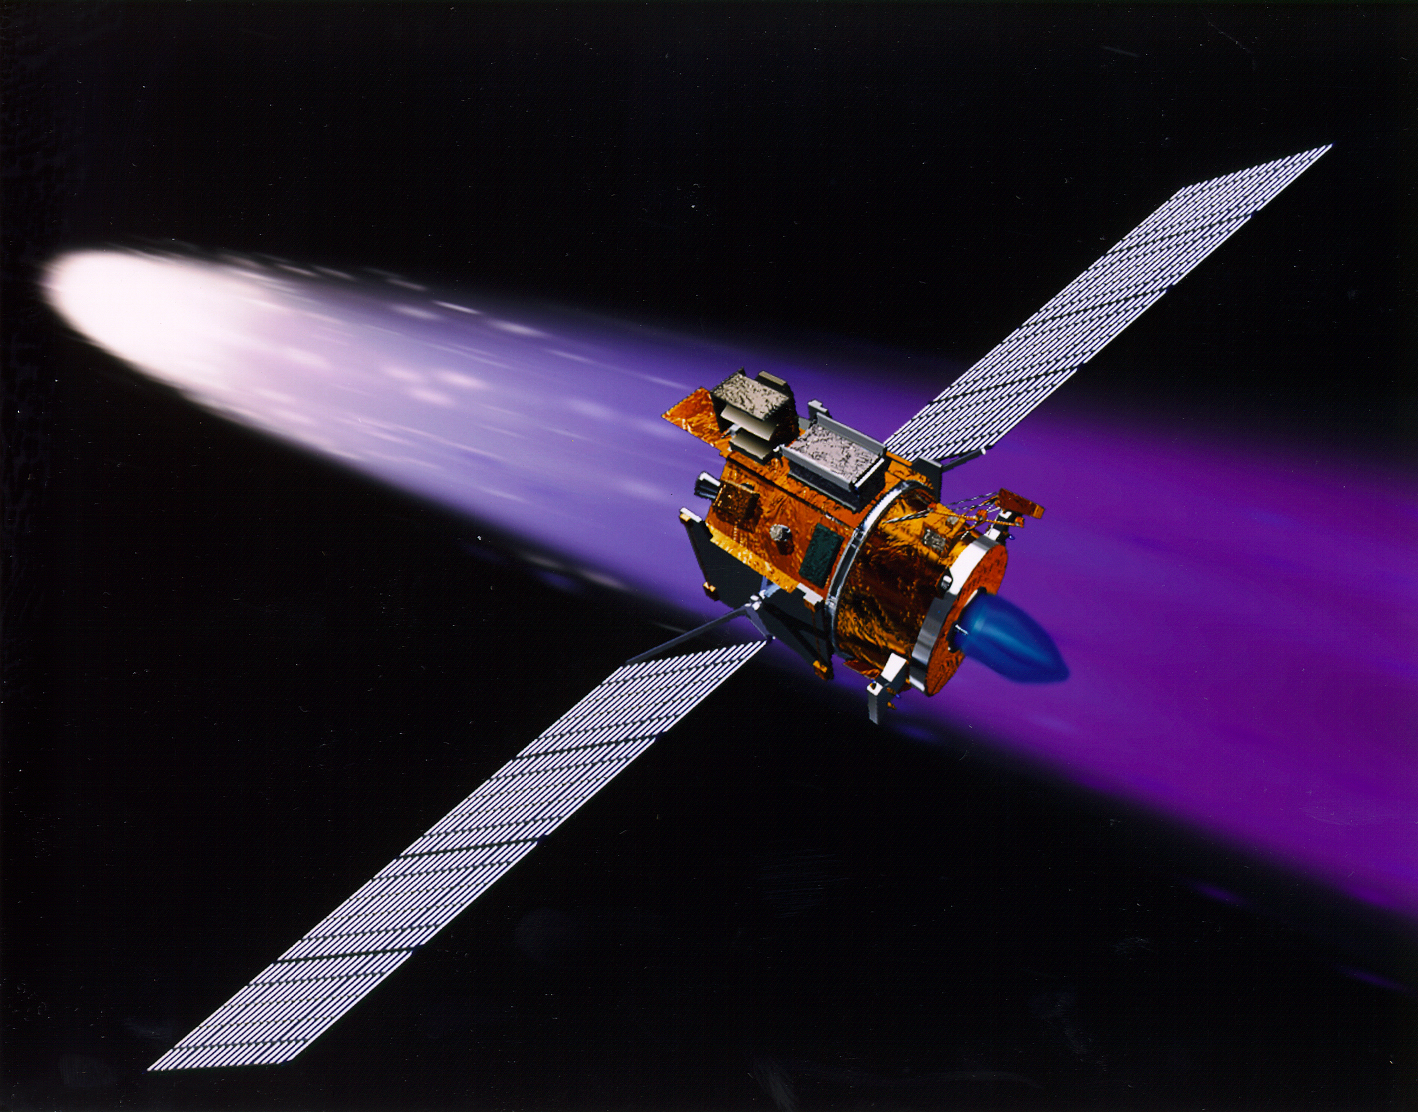
\includegraphics[height=0.4\textheight,width=0.5\textwidth,keepaspectratio]{figures/defense/deepspace1.jpg}
\end{center}
\hyperlink{slide:propulsion}{\beamergotobutton{Ideal Rockets}}
\end{frame}   %-----------------------------%

\subsection[Spacecraft Autonomy]{Spacecraft Autonomy}
% why study the coupled attitude/translational problem

\begin{frame}[t]{Spacecraft Autonomy} %-----------------------------%
\begin{itemize}
    \item Autonomous control of space vehicles is critical
    \begin{itemize}
        \item Avoid extensive planning and interaction by operators
        \item Ability to operate safely with system uncertainty 
        \item Independently navigate hazards and handle possible failures
    \end{itemize}
\end{itemize}
\visible<2>{
\begin{center}
    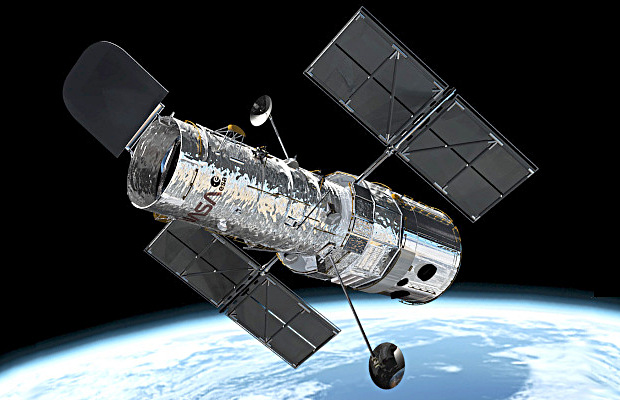
\includegraphics[width=0.5\textwidth,height=0.35\textheight,keepaspectratio]{figures/defense/hubble.jpg}\hfill
    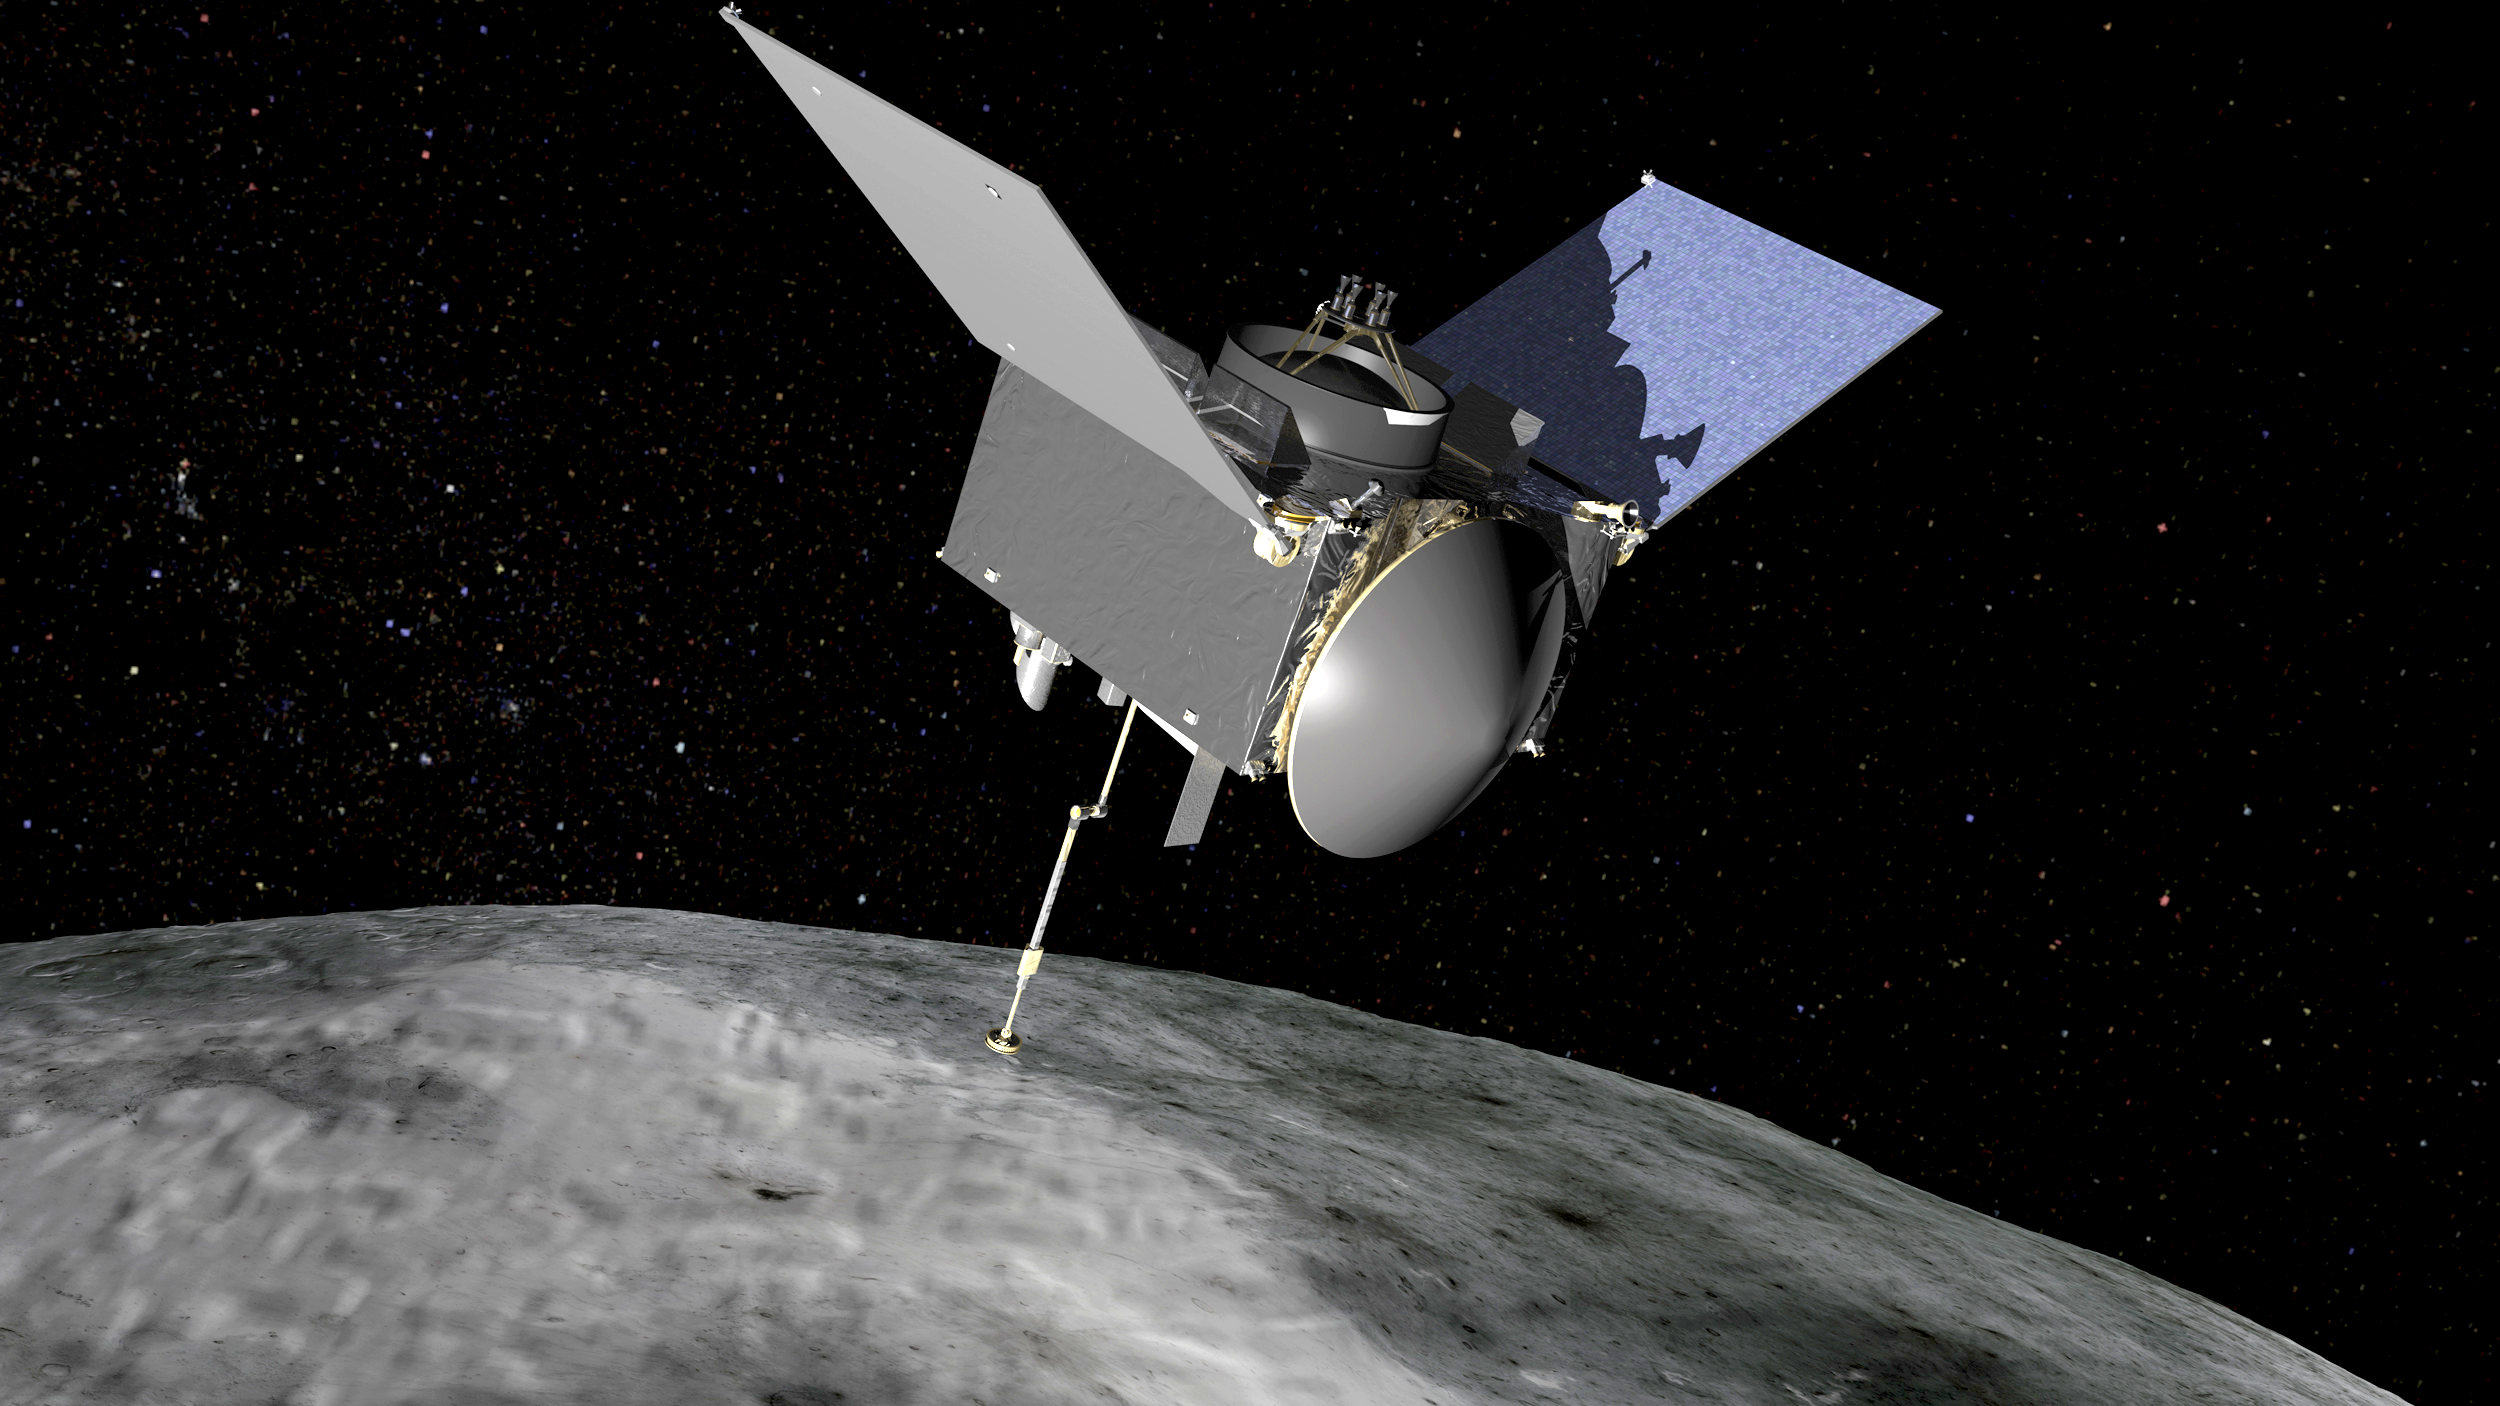
\includegraphics[width=0.5\textwidth,height=0.4\textheight,keepaspectratio]{figures/defense/osires_rex.png}
\end{center}
}
\note[itemize]{
    \item Autonomy is a key component to enable asteroid missions
}
\end{frame}   %-----------------------------%

\begin{frame}[t]{Why send spacecraft to asteroids?}
    \begin{itemize}
        \item<1-> Some properties only available at the asteroid:
            \begin{itemize}
                \item High fidelity gravitational model
                \item Surface samples or return missions
            \end{itemize}
        \item<2-> Gain experience for future missions
            \begin{itemize}
                \item Weak gravitational field allows for less costly manuevers
                \item Asteroid tours for future deep-space human missions
            \end{itemize}
        \item<3-> Avoiding future impacts
            \begin{itemize}
                \item Local spacecraft can aid in ground based tracking
                \item Mitigation: Gravity tractors, kinetic impactors, solar sails
            \end{itemize}
    \end{itemize}

\end{frame}
